\section*{Analysis}
\phantomsection\label{sec:analysis}

\paragraph{Aggregation penalty.} The aggregation penalty ranges from 1.36\pp{} to 19\pp{}, negligible at function level ($\bar{T} \approx 2.3$) but substantial at repo level ($\bar{T} \gg 10$; Appendix~\ref{app:extended_analysis}(a)).

\begin{figure}[t]
\centering
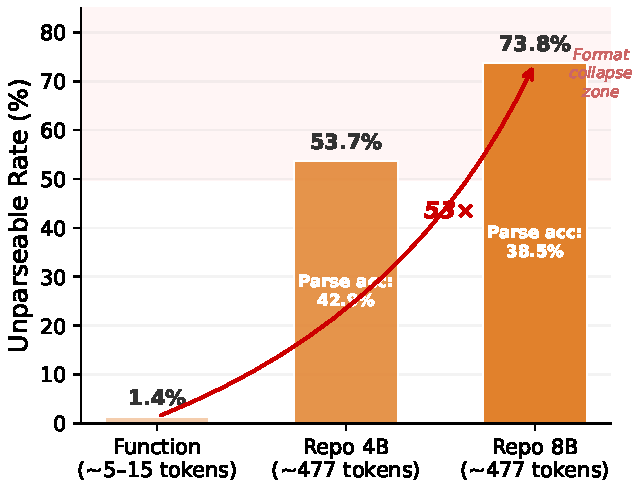
\includegraphics[width=0.72\columnwidth]{figures/paper/fig_cwm_unparseable.pdf}
\caption{\cwm{} unparseable rate by complexity level. Function-level outputs (${\sim}$5--15 tokens) yield 1.4\% unparseable; repo-level outputs (${\sim}$477 tokens) reach 53.7\% (4B) and 73.8\% (8B). Parseable-only accuracy (inside bars) decreases from 4B to 8B despite rising overall accuracy---evidence of default-assignment inflation.}
\label{fig:cwm_unparseable}
\end{figure}

\paragraph{Why does generation degrade at repo level?} Output complexity increases nonlinearly: function-level outputs average ${\sim}$5--15 tokens; repo-level outputs average ${\sim}$477 tokens (Figure~\ref{fig:cwm_unparseable}), leading to format collapse (53--74\% unparseable; Appendix~\ref{app:qualitative}). Even parseable outputs achieve only 38--43\%, below majority; a model accidentally trained on CLS-format data achieves 86.05\% with 0\% unparseable; this confirms that degradation stems from output format complexity, not task difficulty (Appendix~\ref{app:extended_analysis}(c)). Four targeted interventions all fail to close this gap (Appendix~\ref{app:extended_analysis}(g)). \cls{} achieves 217$\times$ higher throughput (1 vs.\ avg 477 output tokens).

\begin{figure}[t]
\centering
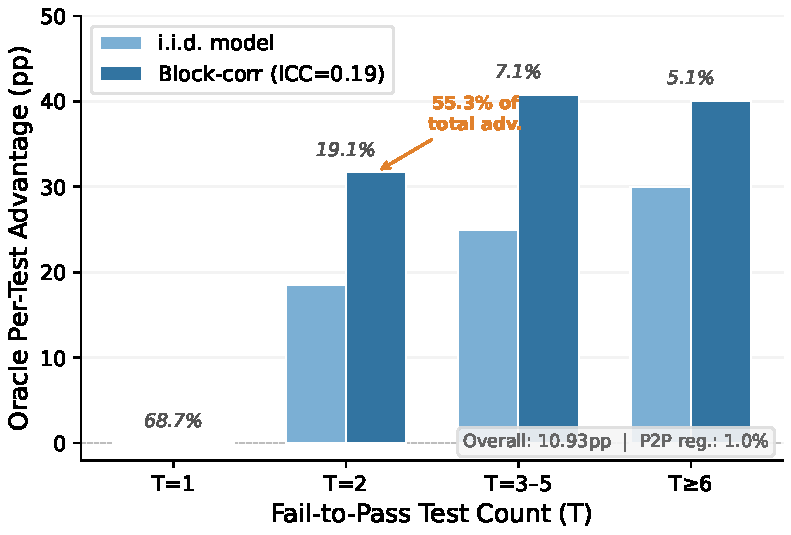
\includegraphics[width=0.82\columnwidth]{figures/paper/fig3_oracle_stratified.pdf}
\caption{Oracle per-test advantage by F2P test count $T$. Advantage is zero at $T{=}1$ (68.7\% of instances) and concentrates at $T{=}2$ (19.1\%, contributing 55.3\% of total advantage).}
\label{fig:oracle_stratified}
\end{figure}

\paragraph{Error complementarity.} \cls{} and \cwm{} make partially complementary errors. An oracle combination achieves 90.63\% (+2.80\pp{}; 95\% CI [89.3\%, 91.9\%]; single-seed) at function level and 95.83\% (+14.58\pp{}; $n{=}48$) at repo level (Figure~\ref{fig:oracle_stratified}). Simple routing heuristics capture $<$0.4\pp{} of the oracle gap; the complementarity is instance-specific, so simple heuristics are insufficient. Whether a learned router can capture this advantage remains open (Appendix~\ref{app:oracle}).

\section*{Threats to Validity}
\phantomsection\label{sec:threats}

We identify five potential confounds (Appendix~\ref{app:threats}): checkpoint selection ($<$1\pp{}), evaluation sequence length (${\sim}$1.5\pp{}), preprocessing (${\sim}$8\pp{}; val-test distribution shift in Appendix~\ref{app:mutation_distribution}), \traj{} training regime, and \cwm{} scale/pretraining (primary limitation). Preprocessing and checkpoint interact, accounting for up to 7.68\pp{} variation within one model (Appendix~\ref{app:threats}). The 18--26\pp{} gap exceeds any single confound, but correlated confounds and limited seeds preclude definitive causal attribution. Holm-Bonferroni ($k{=}5$) confirms the two core claims (adjusted $p{=}0.015$ and $p{=}0.028$; Table~\ref{tab:holm}).

\begin{table}[t]
\centering
\small
\caption{Holm-Bonferroni correction for primary comparisons ($k{=}5$). Comparisons ranked by raw $p$-value; each tested against $\alpha / (k - \text{rank} + 1)$.}
\label{tab:holm}
\setlength{\tabcolsep}{3pt}
\resizebox{\columnwidth}{!}{%
\begin{tabular}{clcccc}
\toprule
\textbf{Rank} & \textbf{Comparison} & \textbf{Raw $p$} & \textbf{Factor} & \textbf{Adj $p$} & \textbf{Sig.?} \\
\midrule
1 & Repo: \cls{} vs \cwm{} & 0.003 & $\times$5 & 0.015 & \checkmark \\
2 & Func: \cls{} vs \cwm{} (TOST $\pm$2\pp{}) & 0.007 & $\times$4 & 0.028 & \checkmark \\
3 & Func: \cls{} vs \traj{} (TOST $\pm$2\pp{}) & 0.025 & $\times$3 & 0.075 & --- \\
4 & Repo: \cwm{} vs \traj{} & 0.039 & $\times$2 & 0.078 & --- \\
5 & Repo: \cls{} vs \traj{} & 0.385 & $\times$1 & 0.385 & --- \\
\bottomrule
\end{tabular}}
\end{table}
